% Pseudo-GT / V-Max SAC progress --- group meeting
% Compile: pdflatex main.tex   (run twice for the TOC / section counters)
%
% Structure:
%   main.tex   -- preamble, title, outline, and \input of the section files
%   7_03.tex   -- July 3 recap (pipeline + first results), kept in full
%   7_17.tex   -- July 17 update (banking, quality, repair, ceiling)
%   7_29.tex   -- July 29 update (ES init-bank diagnosis, SAC init)
\documentclass[aspectratio=169,11pt]{beamer}
\usetheme{Madrid}
\usecolortheme{default}
\usepackage[T1]{fontenc}
\usepackage{lmodern}
\usepackage{amsmath,amssymb}
\usepackage{booktabs}
\usepackage{pifont}          % \ding{55} cross mark
\usepackage{tikz}
\usepackage{graphicx}
\usetikzlibrary{positioning,arrows.meta,shapes,fit,calc}

\graphicspath{{figs/}}

\title{Autonomous Driving Policy: Hard Scenes, Self-Improving}
\subtitle{\small Solving Failure Cases with RL}
\author{Yixi}
\date{July 2026}

% --- shared macros ---------------------------------------------------------
\newcommand{\womdsucc}{\textbf{68\%}}
\newcommand{\trainacc}{\textbf{$\sim$97\%}}
\newcommand{\good}{\textcolor{green!55!black}{\checkmark}}
\newcommand{\bad}{\textcolor{red!70!black}{\ding{55}}}

% Show a progress outline at the start of each section
\AtBeginSection[]{
  \begin{frame}{Outline}
    \tableofcontents[currentsection]
  \end{frame}
}

\begin{document}

% ------------------------------------------------------------------
\begin{frame}
  \titlepage
\end{frame}

\begin{frame}{Outline}
  \tableofcontents
\end{frame}

% ------------------------------------------------------------------
% ==================================================================
% July 3 recap --- kept in full. Frames only; preamble lives in main.tex.
% ==================================================================
\section{Recap: pipeline \& first results (July 3)}

% ------------------------------------------------------------------
\begin{frame}{Motivation}
  \textbf{Goal:} refine trajectories on \emph{hard} VLA failure cases and export clean rollouts for downstream finetuning.

  \vspace{0.6em}
  \begin{itemize}
    \item Train a strong driving policy with \textbf{V-Max SAC} on \textbf{ScenarioMax} (V-Max native layout).
    \item Roll the checkpoint on mapped failure scenarios $\rightarrow$ \textbf{pseudo-GT} trajectories.
    \item Score rollouts with the \textbf{original WOMD / VLA success criterion} (goal + safety).
    \item Use successful rollouts for \textbf{policy / planner finetuning} (next step).
  \end{itemize}
\end{frame}

% ------------------------------------------------------------------
\begin{frame}{V-Max SAC setup (\texttt{repro\_sac\_v2})}
  \begin{columns}[T]
    \column{0.52\textwidth}
    \textbf{Environment}
    \begin{itemize}
      \item Simulator: Waymax via V-Max wrappers
      \item Data: \texttt{ScenarioMax (400K)}
        \begin{itemize}
            \item Converted from WOMD raw data
        \end{itemize}
      \item Dynamics: bicycle model
      \item Horizon: 80 RL steps / episode; 64 agents; 10$\times$300 SDC paths
    \end{itemize}

    \vspace{0.5em}
    \textbf{Algorithm}
    \begin{itemize}
      \item Soft Actor-Critic (SAC), 25M env steps
      \item Gaussian policy, twin Q, $\alpha{=}0.2$
    \end{itemize}

    \column{0.48\textwidth}
    \textbf{Reward (linear)}
    \begin{center}
      \begin{tabular}{@{}lr@{}}
        \toprule
        Term & Weight \\
        \midrule
        overlap & $-1.0$ \\
        offroad & $-1.0$ \\
        run red light & $-1.0$ \\
        off-route & $-0.2$ \\
        progression (route) & $+0.2$ \\
        \midrule
        \multicolumn{2}{l}{\emph{No explicit goal-reaching term}} \\
        \bottomrule
      \end{tabular}
    \end{center}

    Termination: offroad, overlap, run\_red\_light.
  \end{columns}
\end{frame}

% ------------------------------------------------------------------
\begin{frame}{Policy architecture: LQ encoder + MLP head}
  \textbf{Observation} (\texttt{obs\_type=vec}): flat vector unflattened into
  \begin{itemize}
    \item SDC history, 16 closest agents, local roadgraph (200 pts),
          5 traffic lights, 3 SDC path-target waypoints
  \end{itemize}

  \vspace{0.4em}
  \textbf{LQ encoder} (Latent-Query / Perceiver-style):
  \begin{enumerate}
    \item \textbf{Per-modality MLP embed:} 5 separate $[256,256]$ MLPs $\rightarrow d_k{=}64$ + learned positional encodings
    \item \textbf{Scene tokens:} concatenate embedded tokens ($\sim$313) with validity masks
    \item \textbf{LQAttention} ($\times 4$, tied weights): 16 learnable latents attend to scene via cross-attention, then self-attention + feedforward each block
    \item \textbf{Pooling:} mean over 16 latents $\rightarrow$ fixed-size embedding
  \end{enumerate}

  \vspace{0.4em}
  \textbf{Heads:}
  \begin{itemize}
    \item \textbf{Policy MLP} $[256,64,32]$ $\rightarrow$ Gaussian $(a_x, a_\delta)$
    \item \textbf{Twin Q MLPs} $[256,64,32]$ (separate encoders; actions concatenated at input)
  \end{itemize}
\end{frame}

% ------------------------------------------------------------------
\begin{frame}{Training result on ScenarioMax}
  \begin{block}{Native V-Max eval (\texttt{ScenarioMaxWaymoValid})}
    Episode \textbf{accuracy} $\approx$ \trainacc{} over training\\
    \small(accuracy = no offroad, overlap, or red-light termination)
  \end{block}

  \vspace{0.5em}
  Policy learns \textbf{safe route following} on ScenarioMax:
  \begin{itemize}
    \item \texttt{progression} rewards moving along expert SDC paths (arc-length), not Euclidean distance to a goal point.
    \item Strong collision / offroad avoidance on the \emph{training} map layout.
  \end{itemize}

  \vspace{0.3em}
  \centering
  \textit{Good sim driver on ScenarioMax --- but objective $\neq$ WOMD goal-reaching.}
\end{frame}

% ------------------------------------------------------------------
\begin{frame}{Pseudo-GT pipeline}
  {\large\bfseries Scene linking via \texttt{scenario/id}}

  \vspace{0.8em}
  \textbf{Rollout}:\\[0.35em]
  Failure JSON $\rightarrow$ \texttt{tfrecord + scene\_idx}
  $\rightarrow$ read WOMD record $\rightarrow$ \texttt{scenario/id}
  $\rightarrow$ ScenarioMax scene $\rightarrow$ SAC rollout $\rightarrow$ \texttt{trajectory.npz}

  \vspace{0.9em}
  \textbf{Eval}:\\[0.35em]
  Failure JSON $\rightarrow$ \texttt{tfrecord + scene\_idx}
  $\rightarrow$ WOMD scene $\rightarrow$ splice trajectory.npz $\rightarrow$ Metrics
\end{frame}

% ------------------------------------------------------------------
\begin{frame}{Metrics on failure scenarios}
  \begin{table}
    \centering
    \small
    \begin{tabular}{@{}lccp{5.4cm}@{}}
      \toprule
      Metric & Rate & Scene & Meaning \\
      \midrule
      \textbf{Failure success} & \womdsucc{} & WOMD &
        Goal ($\leq$2\,m) + no overlap/offroad/TL before goal \\
      Goal reached & 70\% & WOMD & Ever within 2\,m of \texttt{goal\_xy} \\
      Overlap & 3.7\% & WOMD & Collision with another agent \\
      Offroad & 4.6\% & WOMD & Ego off drivable surface \\
      TL violation & 0.5\% & WOMD & Ran red light \\
      \midrule
      Original VLA success & 0\% & WOMD & Input set (all prior failures) \\
      Still failing & 32\% & WOMD & \\
      \bottomrule
    \end{tabular}
  \end{table}

  \vspace{0.3em}
  \textbf{Takeaway:} \womdsucc{} clean success on hard failures; driving is \textbf{safe}, main gap is \textbf{goal-reaching}.
\end{frame}

% ------------------------------------------------------------------
\begin{frame}{What drives failures?}
  \begin{columns}[T]
    \column{0.48\textwidth}
    \textbf{Among failures (32\%):}
    \begin{itemize}
      \item \textbf{94\%} missed goal (never within 2\,m)
      \item 11\% overlap, 14\% offroad
      \item Only \textbf{4} cases: reached goal but not clean
    \end{itemize}

    \vspace{0.5em}
    \textbf{vs.\ original VLA:}
    \begin{itemize}
      \item VLA reached goal 86\%, but \textbf{never cleanly}
      \item Overlap 34\%, offroad 65\%
      \item SAC: much safer, fewer goals
    \end{itemize}

    \column{0.52\textwidth}
    \textbf{Scenario 052: failure mode comparison}
    \vspace{0.3em}

    \small
    \begin{tabular}{@{}p{1.55cm}p{4.8cm}@{}}
      \toprule
      & \textbf{VLA} \emph{(failed: offroad)} \\
      \midrule
      Driving & Crosses \textbf{road boundary}; aggressive \\
      Speed & Fast \\
      Goal & \checkmark\ Reached (0.02\,m) \\
      \midrule
      & \textbf{RL / SAC} \emph{(failed: goal miss)} \\
      \midrule
      Driving & Stays in lane; avoids boundary \\
      Speed & Slow / cautious \\
      Goal & \textbf{11.5\,m} from goal (threshold 2\,m) \\
      \bottomrule
    \end{tabular}

    \vspace{0.5em}
    \textit{Same scene, opposite failure modes: VLA rushes to goal offroad; RL drives safely but stops short.}
  \end{columns}
\end{frame}

% ------------------------------------------------------------------
\begin{frame}{Training objective vs.\ WOMD eval}
  \centering
  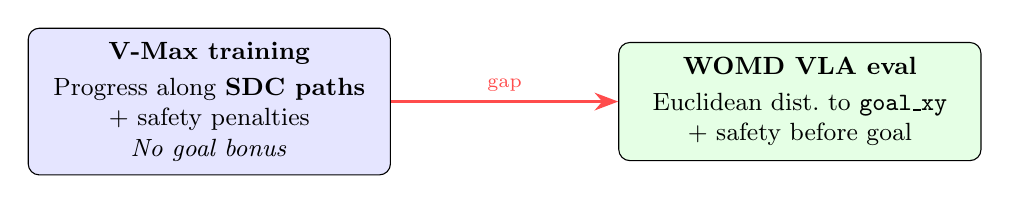
\begin{tikzpicture}[
    box/.style={draw, rounded corners, align=center, font=\small,
                minimum width=4.6cm, minimum height=1.5cm, inner sep=5pt}
  ]
    \node[box, fill=blue!10] (train) at (0,0) {
      \textbf{V-Max training}\\[2pt]
      Progress along \textbf{SDC paths}\\
      $+$ safety penalties\\
      \emph{No goal bonus}
    };
    \node[box, fill=green!10] (eval) at (7.5,0) {
      \textbf{WOMD VLA eval}\\[2pt]
      Euclidean dist.\ to \texttt{goal\_xy}\\
      $+$ safety before goal
    };
    \draw[-{Stealth[length=3mm]}, thick, red!70] (train.east) -- node[above, font=\scriptsize]{gap} (eval.west);
  \end{tikzpicture}

  \vspace{0.8em}
  \begin{itemize}
    \item Remaining \textbf{32\%} WOMD failures are mostly \textbf{goal miss}, not crashes.
    \item Scenario 052 pattern: clean driving, 11\,m from goal; VLA reached goal offroad.
  \end{itemize}
\end{frame}

% ------------------------------------------------------------------
\begin{frame}{Real difficulty gap}
  \centering
  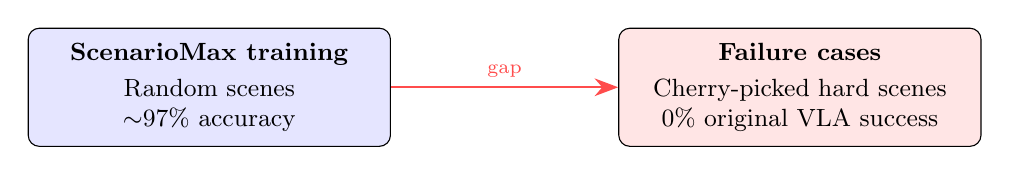
\begin{tikzpicture}[
    box/.style={draw, rounded corners, align=center, font=\small,
                minimum width=4.6cm, minimum height=1.5cm, inner sep=5pt}
  ]
    \node[box, fill=blue!10] (train) at (0,0) {
      \textbf{ScenarioMax training}\\[2pt]
      Random scenes\\
      $\sim$97\% accuracy
    };
    \node[box, fill=red!10] (fail) at (7.5,0) {
      \textbf{Failure cases}\\[2pt]
      Cherry-picked hard scenes\\
      0\% original VLA success
    };
    \draw[-{Stealth[length=3mm]}, thick, red!70] (train.east) -- node[above, font=\scriptsize]{gap} (fail.west);
  \end{tikzpicture}

  \vspace{0.8em}
  \begin{itemize}
    \item Real hazards concentrate here: \textbf{overlap} (3.7\%), \textbf{offroad} (4.6\%) on WOMD eval.
    \item Original VLA was much worse: 34\% overlap, 65\% offroad --- policy must handle tight interactions.
    \item \textbf{Solution:} finetune (overfit) on \textbf{failure scenes only}; early stop on \textbf{both}
          eval scenes (general driving) and failure scenes (learn those layouts).
  \end{itemize}
\end{frame}

% ------------------------------------------------------------------
\begin{frame}{Next steps (as planned July 3)}
  \begin{enumerate}
    \item \textbf{Add goal-reaching reward} to V-Max training / finetuning
    \begin{itemize}
      \item e.g.\ bonus for reducing distance to expert \texttt{goal\_xy} (or route endpoint)
      \item Finetune \texttt{repro\_sac\_v2} on failure subset with goal term
    \end{itemize}
    \item \textbf{Finetune on only Failure Scenes}. Early stop jointly with eval scenes and failure scenes to prevent overfitting bad driving behaviors
    \item \textbf{Export clean rollouts} for downstream \textbf{policy / planner finetuning}
    \begin{itemize}
      \item Diffusion planner or VLA refinement on successful trajectories
    \end{itemize}
  \end{enumerate}

  \vspace{0.6em}
  \centering
  \textit{$\Rightarrow$ July 17: all three done. The goal reward closed most of the gap ---
  and the real work became \textbf{pseudo-GT quality}.}
\end{frame}

% ==================================================================
% July 17 update. Frames only; preamble lives in main.tex.
% ==================================================================

% ##################################################################
\section{The failure set is mostly already solved}
% ##################################################################

% ------------------------------------------------------------------
\begin{frame}{Since July 3: the goal-reaching reward}
  July 3's plan was ``add a goal term.'' Done --- two pieces:
  \begin{itemize}
    \item \textbf{\texttt{reached\_goal\_once}} $+5$: one-off bonus the first time the SDC is within 2\,m of the goal (cannot be farmed by camping).
    \item \textbf{Potential-based goal shaping}: $\Phi(s) = -\,\text{dist to goal}$, dense and policy-invariant (Ng et al.\ 1999).
  \end{itemize}

  \vspace{0.6em}
  \centering
  \textit{This closed most of the goal-reaching gap --- but the interesting part is what happened next.}
\end{frame}

% ------------------------------------------------------------------
\begin{frame}{The failures are mostly already solved}
  \textbf{Clean-rollout banking}, warm-started from the pretrained checkpoint:
  \begin{center}
    \begin{tabular}{@{}lc@{}}
      \toprule
      & solved (clean, goal-reaching) \\
      \midrule
      pretrained checkpoint, \emph{first} eval & \textbf{157 / 218} ($\sim$72\%) \\
      after 20k SAC steps & \textbf{202 / 218} (92.7\%) \\
      \bottomrule
    \end{tabular}
  \end{center}

  \vspace{0.5em}
  \textbf{Reframe:} these 245 scenes are the \emph{diffusion / VLA planner's} failures ---
  harvested from \emph{it} failing, not V-Max.
  \begin{itemize}
    \item V-Max SAC pretrain is $\sim$95\% clean on validation; nothing here is adversarial to it.
    \item $\sim$72\% already solved by the \textbf{pre-trained SAC policy}, before any failure-set finetuning. Only the residual deserves budget.
  \end{itemize}
\end{frame}

% ##################################################################
\section{Harvesting pseudo-GTs: the trajectory bank}
% ##################################################################

% ------------------------------------------------------------------
\begin{frame}{Banking: success is a union over time}
  \textbf{Idea:} a scenario only has to succeed \emph{once}, at \emph{any} checkpoint ---
  not all-clean at one moment.
  \begin{itemize}
    \item Evaluate periodically; the first time a scene comes out clean, write its
          trajectory to disk and mark it banked.
    \item SAC oscillating between scenes (solve A, drift, solve B) becomes the
          \textbf{harvest mechanism}, not a failure mode.
    \item Banked scenes drop out of training $\rightarrow$ budget flows to the unsolved ones.
    \item Keep the \emph{smoothest} clean rollout seen per scene (upgrade in place).
  \end{itemize}

  \vspace{0.5em}
  \textbf{Clean} $=$ reached goal $\wedge\ \neg$offroad $\wedge\ \neg$overlap ---
  \emph{identical} to the raw VLA failure label (verified on all 245).
\end{frame}

% ##################################################################
\section{But the rollouts are not clean BC targets}
% ##################################################################

% ------------------------------------------------------------------
\begin{frame}{Problem 1 --- overshoot}
  Banked rollouts reach the goal, then \textbf{keep driving}.
  \begin{itemize}
    \item Median \textbf{33\,m} past the goal (max 75\,m), $\sim$3\,s of extra driving.
    \item Clean by the metric (\texttt{reached\_goal} = ``reached at least once'').
  \end{itemize}

  \vspace{0.4em}
  \textbf{Why:} the expert log does \emph{not} decelerate into the goal.
  \begin{itemize}
    \item The goal is just where the 9\,s recording was \emph{cut} ---
          the human is still moving \textbf{6.8\,m/s} (median) at the last logged frame.
    \item So a good pseudo-GT should be \textbf{truncated} at closest approach, not run to 91 frames.
  \end{itemize}
\end{frame}

% ------------------------------------------------------------------
\begin{frame}{Problem 2 --- the ``shimmy''}
  \begin{columns}[T]
    \column{0.46\textwidth}
    A \textbf{period-2 yaw limit cycle}: heading flips $\pm25^\circ$ \emph{every frame}
    while the body tracks a straight path.
    \begin{itemize}
      \item Peak yaw rate \textbf{3.07\,rad/s} (p50) vs the human's \textbf{0.35} (max ever 1.09).
      \item \textbf{186 / 202} rollouts sit outside the human's \emph{entire} yaw-rate range.
      \item $\sim$21\% in a severe sustained cycle.
    \end{itemize}
    \textbf{Cause:} nothing penalizes it, and entropy $\alpha$ collapsed toward a bang-bang policy.

    \column{0.54\textwidth}
    \centering
    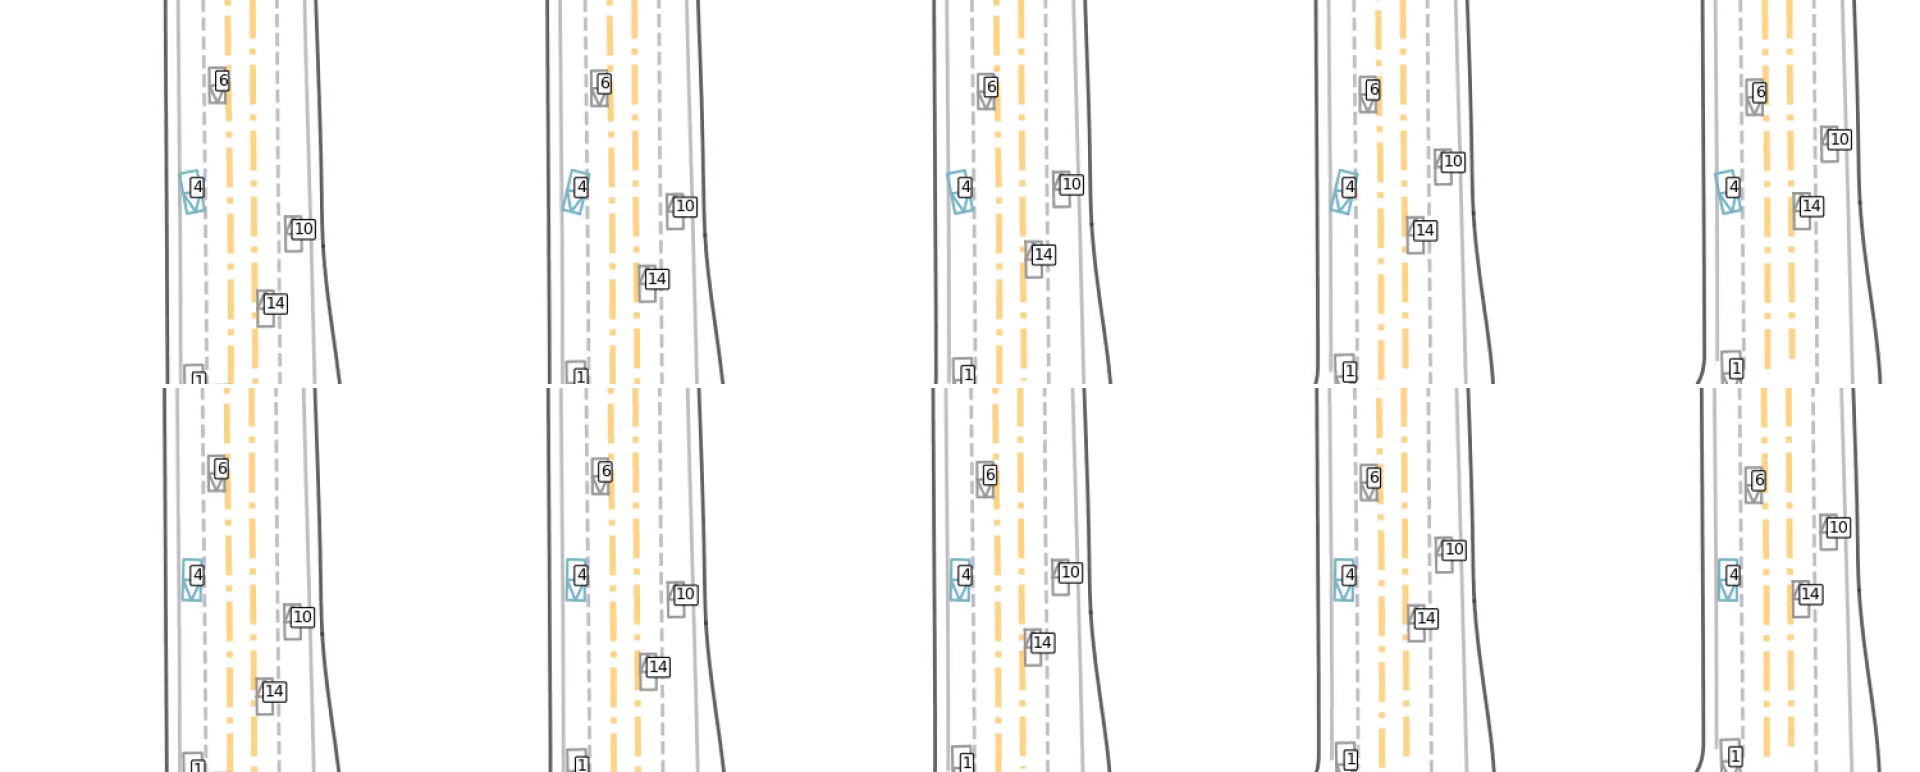
\includegraphics[width=\linewidth]{shimmy_repair_197}\\[2pt]
    {\scriptsize Consecutive frames. \textbf{Top:} original --- the ego box tilts a
    different way each frame. \textbf{Bottom:} repaired (next section).}
  \end{columns}
\end{frame}

% ##################################################################
\section{Fixing pseudo-GT quality}
% ##################################################################

% ------------------------------------------------------------------
\begin{frame}{Fix 1 --- truncate at the goal}
  Cut each trajectory at its closest approach to the goal.
  \begin{center}
    \begin{tabular}{@{}lcc@{}}
      \toprule
      distance to goal at last frame & before & after \\
      \midrule
      median & 33\,m & \textbf{0.7\,m} \\
      \bottomrule
    \end{tabular}
  \end{center}

  \vspace{0.5em}
  \textbf{Truncate by validity, not by shortening the array.}
  \begin{itemize}
    \item Every splice path forces \texttt{valid=True} only on the written slice;
          a shortened array leaves the \emph{original} human log in the tail.
    \item Measured teleport if done wrong: \textbf{16.7\,m in one 0.1\,s frame}
          (vs a normal 1.4\,m step). So: set \texttt{valid=False} past the cut.
  \end{itemize}
\end{frame}

% ------------------------------------------------------------------
\begin{frame}{Fix 2 --- can a reward remove the shimmy? No.}
  Added a \texttt{yaw\_rate\_penalty}; swept the weight (same checkpoint, same step):
  \begin{center}
    \small
    \begin{tabular}{@{}lccc@{}}
      \toprule
      penalty & reached rate & frac.\ over 0.95\,rad/s & banked \\
      \midrule
      none    & 0.83 $\to$ \textbf{0.89} & $\sim$0.92 & --- \\
      $-0.5$  & 0.79 $\to$ 0.73          & 0.927      & 0.88 \\
      $-2.0$  & 0.66 $\to$ \textbf{0.45} & 0.962      & 0.72 \\
      \bottomrule
    \end{tabular}
  \end{center}

  \vspace{0.4em}
  \textbf{All cost, no benefit:} the penalty costs goal-reaching and barely moves the chatter;
  at $-2.0$ it \emph{halves} goal-reaching.
  \begin{itemize}
    \item V-Max's own \texttt{comfort} reward is \emph{blind} to it: it savgol-filters yaw,
          which erases a period-2 signal (reads 4.5\,rad/s as 0.06).
    \item[$\Rightarrow$] Fix the artifact \textbf{post-hoc}, not in the reward.
  \end{itemize}
\end{frame}

% ------------------------------------------------------------------
\begin{frame}{Fix 3 --- post-hoc repair}
  \begin{columns}[T]
    \column{0.5\textwidth}
    \textbf{\texttt{path\_savgol}}: smooth the path, then re-derive heading \emph{and} velocity from it.
    \begin{itemize}
      \item The bicycle model bakes the wobble into position ($\pm$0.3\,m), so smoothing
            the \emph{path} beats smoothing yaw alone.
      \item Yaw-reversal rate \textbf{0.50 $\to$ 0.13} (human 0.05); moves the car $\leq$\,0.35\,m.
      \item \textbf{Validated safe} (re-scored on WOMD): 19/20 clean before, \textbf{19/20 after, 0 broken}.
    \end{itemize}

    \vspace{0.2em}
    \centering\small
    \begin{tabular}{@{}lc@{}}
      \toprule
      peak yaw rate (p50, rad/s) & \\
      \midrule
      raw banked rollout & 3.07 \\
      $+$ repair & 1.30 \\
      $+$ keep smoothest per scene & \textbf{0.85} \\
      \midrule
      comfort limit / human & 0.95 / 0.35 \\
      \bottomrule
    \end{tabular}

    \column{0.5\textwidth}
    \centering
    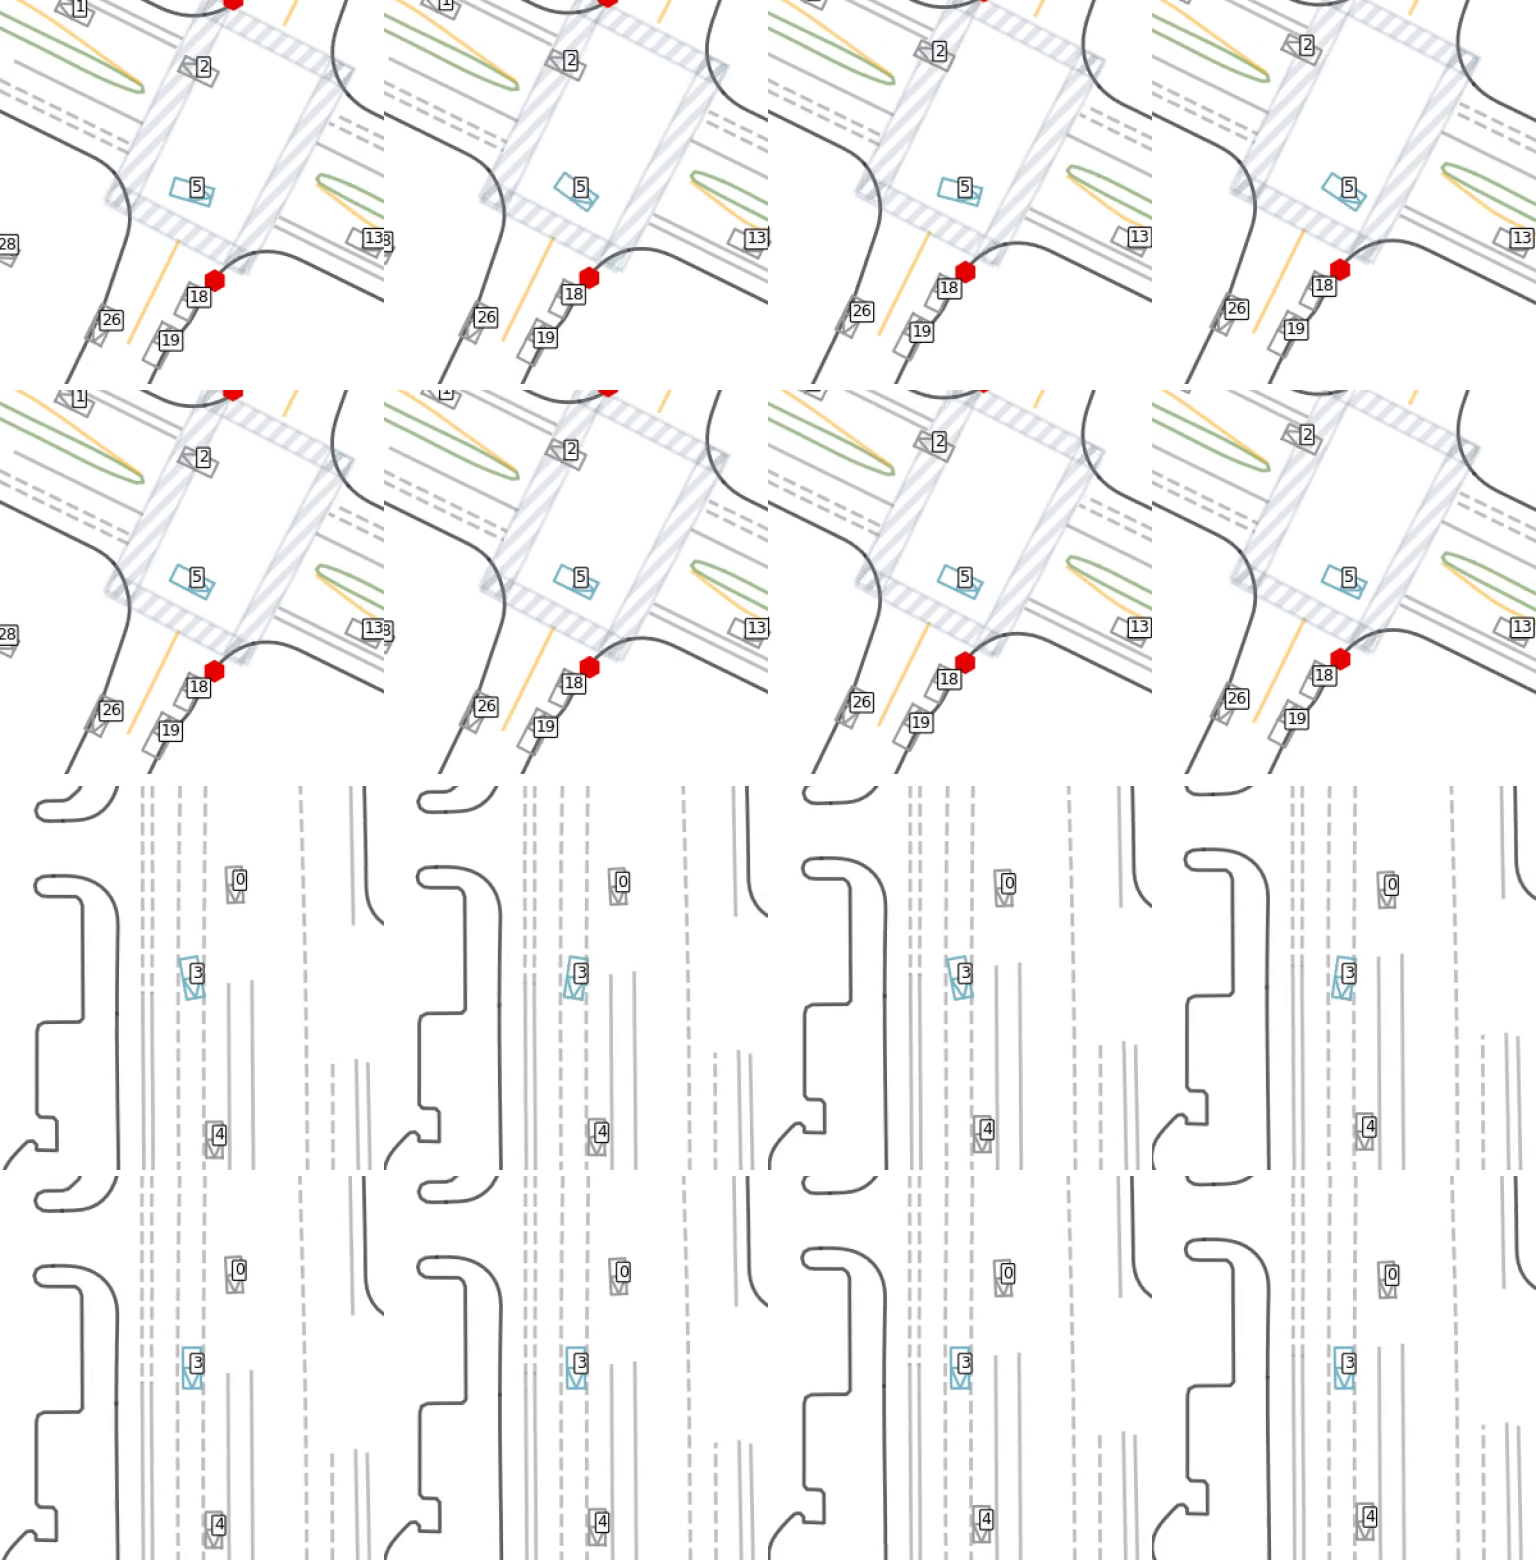
\includegraphics[width=\linewidth]{shimmy_repair_127_149}\\[2pt]
    {\scriptsize Two scenes. In each pair, \textbf{top} original wobbles frame-to-frame,
    \textbf{bottom} repaired stays lane-aligned.}
  \end{columns}
\end{frame}

% ##################################################################
\section{Where we land, and the open issue}
% ##################################################################

% ------------------------------------------------------------------
\begin{frame}{Final accounting: 207 banked, and the residual}
  \begin{columns}[T]
    \column{0.42\textwidth}
    \begin{center}
      \begin{tabular}{@{}lr@{}}
        \toprule
        raw failure scenes & 245 \\
        $-$ overpass (excluded) & $-27$ \\
        \midrule
        in the pipeline & \textbf{218} \\
        clean pseudo-GT banked & \textbf{207} \\
        unbanked & \textbf{11} \\
        \bottomrule
      \end{tabular}
    \end{center}
    \centering\small
    The \textbf{11 unbanked} split into\\ \textbf{8 mislabeled} $+$ \textbf{3 correctly labeled}.

    \column{0.58\textwidth}
    \textbf{The caveats, in full}
    \begin{itemize}
      \item \textbf{27 overpasses} (11\%): ScenarioMax's 2D roadgraph can't stack decks.
            \good\ \textbf{22} recoverable (keep-ego-level filter) $\Rightarrow$ \textbf{240}.
      \item \textbf{Mislabeled} $=$ the \emph{expert log itself} fails the metric (human
            offroad/overlap). \textbf{18} scenes total; verified: log fails \textbf{72.7\%}
            on unbanked vs \textbf{4.8\%} on banked --- concentrated, not noise.
        \begin{itemize}
          \item[\good] \textbf{10} of the 18 we \emph{solved anyway} (policy $>$ human).
          \item[$\cdot$] \textbf{8} still unbanked --- broken label, e.g.\ one is a corrupt $+101$\,m record.
        \end{itemize}
      \item \textbf{3 correctly labeled}: clean expert log, genuinely winnable --- get targeted budget.
    \end{itemize}
    \vspace{0.1em}
    {\scriptsize $\Rightarrow$ practical ceiling $\approx \mathbf{210}$ (207 $+$ the 3); recovering overpasses lifts the denominator to 240.}
  \end{columns}
\end{frame}

% ------------------------------------------------------------------
\begin{frame}{The label is the problem, not the scene}
  On \textbf{10} scenes the \emph{human's own logged trajectory} goes offroad or collides ---
  yet our policy drives them clean and they are banked.
  \begin{columns}[T]
    \column{0.5\textwidth}
    \centering
    \textbf{Expert log (the ``ground truth'')}\\[2pt]
    \includegraphics[width=\linewidth]{mislabeled_expert}\\[2pt]
    {\scriptsize goes offroad / collides}
    \column{0.5\textwidth}
    \centering
    \textbf{Our banked pseudo-GT}\\[2pt]
    \includegraphics[width=\linewidth]{mislabeled_ours}\\[2pt]
    {\scriptsize same scene, driven clean}
  \end{columns}
  \vspace{0.3em}
  \centering\small
  \textit{This is why ``expert log fails'' means \textbf{mislabeled}, not unsolvable.}
\end{frame}

% ------------------------------------------------------------------
\begin{frame}{The open issue: speeding}
  The banked rollouts drive the \emph{right route} --- just too fast.
  \begin{itemize}
    \item Policy vs expert \textbf{path length} to the goal: ratio \textbf{1.00} (median) --- same route.
    \item Reaches the goal at \textbf{$\sim$1.7$\times$ the expert's speed}.
      \begin{itemize}
        \item \emph{median of the per-scene speed ratio} (policy speed at goal / expert speed at goal).
        \item Robust statistic: the \emph{mean} is unusable --- some experts stop \emph{at} the goal, so the ratio blows up.
        \item Equivalently: covers the route in $\sim$60\% of the expert's time (time-compression 1.68$\times$).
      \end{itemize}
    \item The overshoot (Problem 1) is the \emph{symptom}; this is the cause.
  \end{itemize}

  \vspace{0.3em}
  \centering
  \textit{Truncation and repair don't touch this --- it needs reward / episode design
  (the goal is a fixed-\emph{time} budget the policy is rewarded for beating).}
\end{frame}

% ##################################################################
\section{Next steps}
% ##################################################################

% ------------------------------------------------------------------
\begin{frame}{Next steps}
  \begin{enumerate}
    \item \textbf{Distill the harvest.} 207 truncated, repaired pseudo-GTs (yaw $\leq$ human limit)
          $\rightarrow$ finetune the \textbf{diffusion planner}. ScenarioMax$\to$WOMD translation
          verified at \textbf{99.5\%}.
    \item \textbf{Fix the speeding.} The one defect truncation + repair don't touch ---
          reward / episode design (goal as a fixed-time budget the policy beats).
    \item \textbf{Recover the overpasses.} Keep-ego-level pre-filter $\rightarrow$ denominator
          \textbf{240}; the 3 winnable stragglers get targeted budget.
  \end{enumerate}

  \vspace{0.6em}
  \centering
  \textit{From ``68\% clean success'' to a repaired, near-complete pseudo-GT set ---
  ready for downstream finetuning.}
\end{frame}

% ==================================================================
% July 29 update. Frames only; preamble lives in main.tex.
% ==================================================================

% ##################################################################
\section{ES init-bank diagnosis: diffusion vs.\ SAC}
% ##################################################################

% ------------------------------------------------------------------
\begin{frame}{Diagnosis: initialization is bimodal, not gradually deficient}
  \small
  \begin{columns}[T]
    \column{0.46\textwidth}
    \centering
    \begin{tabular}{@{}lrr@{}}
      \toprule
      safe in kept 64 & replans & share \\
      \midrule
      0     & 157 & \textbf{54.5\%} \\
      1--4  &   3 & 1.0\% \\
      33--63&   2 & 0.7\% \\
      64    & 126 & \textbf{43.8\%} \\
      \bottomrule
    \end{tabular}

    \vspace{0.5em}
    288 replans; mean $28.4$, median \textbf{0}.

    \column{0.54\textwidth}
    \begin{itemize}
      \item If the 256-candidate bank contains safes, down-selection keeps
            \textbf{62.5/64 safe} on average; otherwise it keeps
            \textbf{0/64}.
      \item Therefore the main deficiency is a \textbf{replan-level coverage
            collapse}: the proposal bank usually supplies either hundreds of
            safe options or none.
      \item A zero-safe replan raises risk but is not deterministically fatal:
            \textbf{13/22 successes} recovered after at least one.
      \item Both no-goal failures always had safes:
            \textbf{insufficient progress is a separate mode}.
    \end{itemize}
  \end{columns}
\end{frame}

% ------------------------------------------------------------------
\begin{frame}{SAC init closes the coverage collapse}
  \small
  \begin{columns}[T]
    \column{0.46\textwidth}
    \centering
    \begin{tabular}{@{}lrr@{}}
      \toprule
      safe in kept 64 & scenes & share \\
      \midrule
      0   &  2 & \textbf{6.9\%} \\
      64  & 27 & \textbf{93.1\%} \\
      \bottomrule
    \end{tabular}

    \vspace{0.5em}
    29 ES scenes, $K{=}64$ stochastic SAC seeds each; mean \textbf{59.6}/64 safe.

    \column{0.54\textwidth}
    \begin{itemize}
      \item Same bimodal shape, but the \textbf{0-safe mass collapses}:
            \textbf{54.5\% $\to$ 6.9\%} of instances.
      \item Diffusion has to \emph{sample into} a safe mode each draw;
            the offline SAC bank is safe \textbf{by construction} from a
            closed-loop rollout, so coverage no longer depends on that draw.
      \item The 2 remaining 0/64 scenes are not unlucky sampling ---
            \textbf{all 64 seeds fail identically} (one pure overlap, one
            pure offroad): genuinely hard scenes, not a coverage gap.
      \item Caveat: this is per-\textbf{scene} (closed-loop from $t{=}0$),
            not per-\textbf{replan} like the diffusion table --- directionally
            comparable, not the same denominator.
    \end{itemize}
  \end{columns}
\end{frame}


\end{document}
